To use bilevel planning at evaluation time, we must learn predicates, operators, and samplers at training time.
We use the methods of~\citet{chitnis2021learning} for operator learning and sampler learning; see \secref{subsec:oplearning} and \secref{subsec:samplerlearning} for descriptions.
For what follows, it is important to understand that operator learning is fast ($O(|\D|)$), but sampler learning is slow, and both require a given set of predicates.
Our main contribution is a method for predicate invention that precedes operator and sampler learning in the training pipeline.

\begin{algorithm}[t]
  \SetAlgoNoEnd
  \DontPrintSemicolon
  \SetKwFunction{algo}{algo}\SetKwFunction{proc}{proc}
  \SetKwProg{myalg}{}{}{}
  \SetKwProg{myproc}{Subroutine}{}{}
  \SetKw{Continue}{continue}
  \SetKw{Break}{break}
  \SetKw{Return}{return}
  \SetKwFor{For}{for}{}{}
  \myalg{\textsc{ETPT(}{\color{blue} $x_0$, $g$, $\Psi$, $\Omega$}, $\pi^*$\textsc{)}}{
  \tcp{\footnotesize Note: does not take in samplers!}
  \tcp{\footnotesize Parameters: {\color{blue} $n_{\text{abstract}}$},  $t_{\text{upper}}$.}
    \nl {\color{blue} $s_0 \gets \textsc{Abstract}(x_0, \Psi)$\;}
    \nl  $p_{\text{terminate}} \gets 0.0$\;
    \nl  $t_{\text{expected}} \gets 0.0$\;
    \nl \For{{\color{blue} $\hat{\pi}$ in \textsc{GenAbstractPlan}($s_0$, $g$, $\Omega$, $n_{\text{abstract}}$)}}
    {
    \nl $p_{\text{refined}} \gets$ \textsc{EstimateRefineProb($\hat{\pi}$, $\pi^*$)}\;
    \nl  $p_{\text{terminate}} \gets (1 - p_{\text{terminate}})\cdot p_{\text{refined}}$\;
    \nl  $t_{\text{iter}} \gets$ \textsc{EstimateTime({\color{blue}$\hat{\pi}$, $x_0$, $\Psi$}, $\operators$}) \;
    \nl  $t_{\text{expected}} \gets t_{\text{expected}} + p_{\text{terminate}}\cdot t_{\text{iter}}$}
    \nl $t_{\text{expected}} \gets t_{\text{expected}}  + (1 - p_{\text{terminate}})\cdot t_{\text{upper}}  $\;
    \nl \textbf{return} $t_{\text{expected}}$}\;
\caption{\small{Pseudocode for Estimate Total Planning Time in our predicate invention surrogate objective. Commonalities with \algref{alg:plan} are shown in blue. See \secref{sec:learning} for details.}}
\label{alg:surrogate}
\end{algorithm}



Inspired by prior work~\cite{bonet2019learning,loula2019discovering,curtis2021discovering}, we approach the predicate invention problem from a program synthesis perspective~\cite{stahl1993predicate,lavrac1994inductive,cropper2016learning,ellis2020dreamcoder}.
First, we define a compact representation of an infinite space of predicates in the form of a \emph{grammar}.
We then enumerate a large pool of \emph{candidate predicates} from this grammar, with simpler candidates enumerated first.
Next, we perform a \emph{local search} over subsets of candidates, with the aim of identifying a good final subset to use as $\Psi$.
The crucial question in this step is: what \emph{objective function} should we use to guide the search over candidate predicate sets?

\begin{figure*}[t]
  \centering
    \noindent
    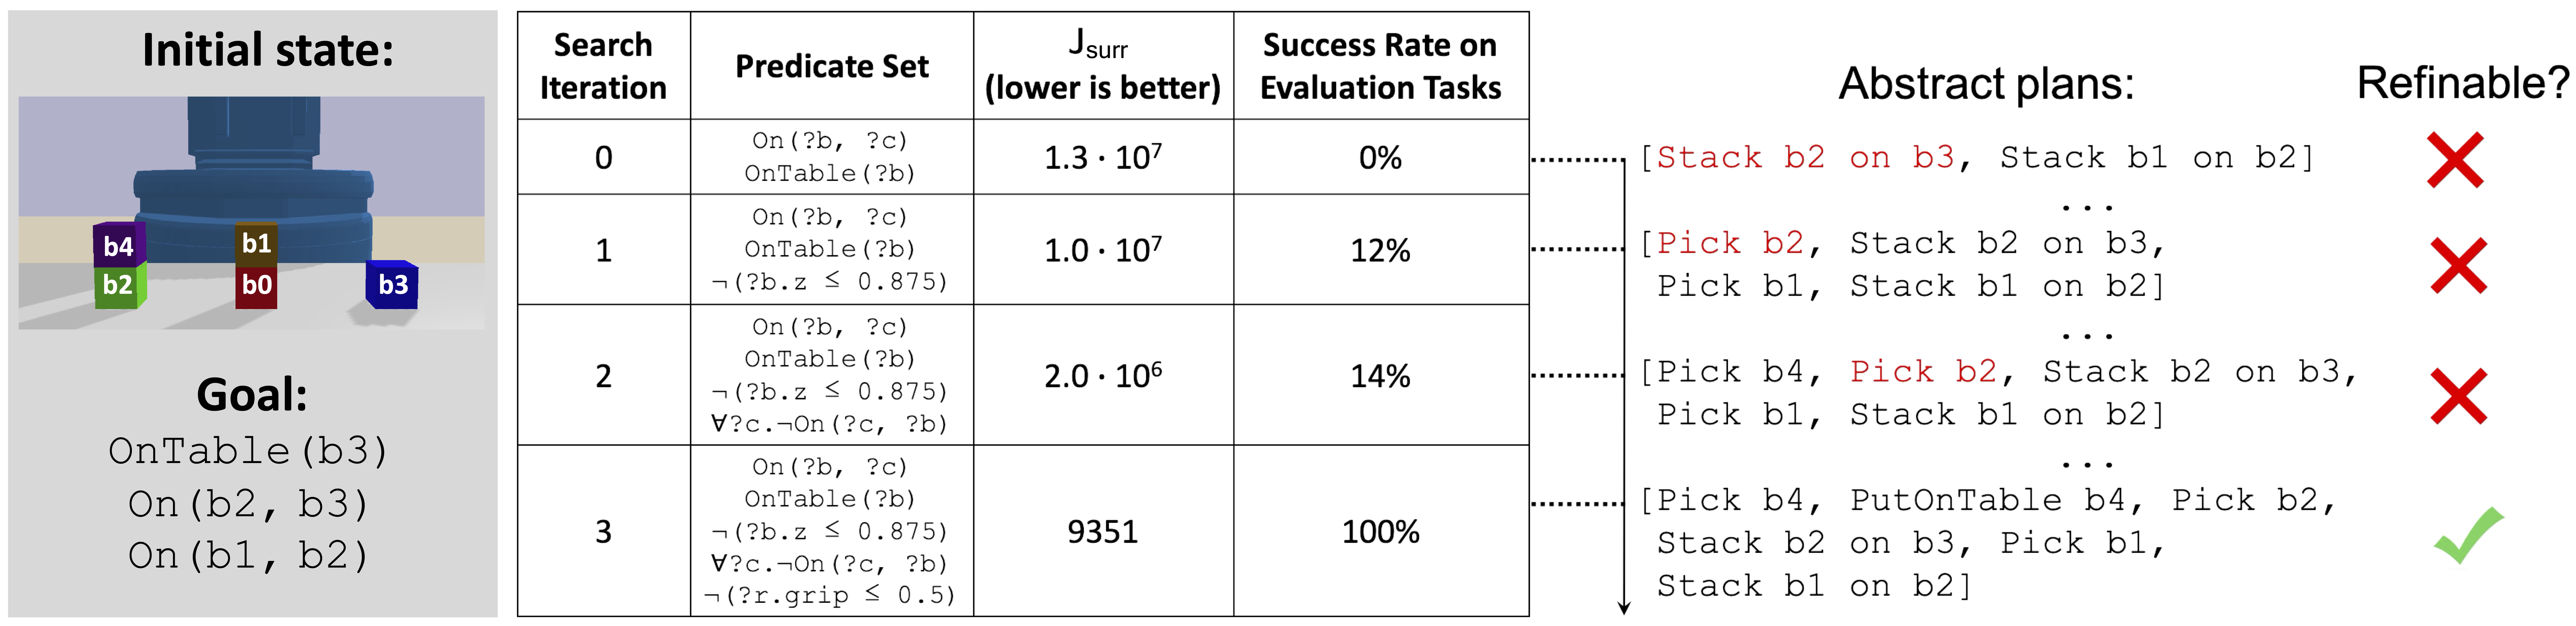
\includegraphics[width=\textwidth]{figures/hill_climbing.png}
    \caption{\small{\textbf{Predicate invention via hill climbing}. (Left) An example task in Blocks. (Middle) Hill climbing over predicate sets, starting with the goal predicates $\Psi_G$. On each iteration, the single predicate that improves $J_{\text{surr}}$ the most is added to the set. The rightmost table column shows success rates on held-out evaluation tasks.
    Each iteration of hill climbing adds a predicate that causes all abstract plans above the dotted line to be pruned from consideration. At iteration 0, the robot believes it can achieve the goal by simply stacking \texttt{b2} on \texttt{b3} and \texttt{b1} on \texttt{b2}, even though it hasn't picked up either block. The first step of this abstract plan (shown in red) is thus unrefinable. At iteration 1, a predicate with the intuitive meaning \texttt{Holding} is added, which makes the A$^*$ only consider abstract plans that pick up blocks before stacking them. Still, the abstract plan shown is unrefinable on the first step because \texttt{b4} is obstructing \texttt{b2} in the initial state. At iteration 2, a predicate with the intuitive meaning \texttt{NothingAbove} is added, which allows the agent to realize that it must move \texttt{b4} out of the way if it wants to pick up \texttt{b2}. This plan is still unrefinable, though: the second step fails, because the abstraction still does not recognize that the robot cannot be holding two blocks simultaneously. Finally, at iteration 3, a predicate with the intuitive meaning \texttt{HandEmpty} is added, and planning succeeds.
    }}
  \label{fig:hill_climbing}
\end{figure*}

\subsection{Scoring a Candidate Predicate Set}
\label{subsubsec:scorefunc}

Ultimately, we want to find a set of predicates $\Psi$ that will lead to efficient planning, after we use the predicates to learn operators $\operators$ and samplers $\samplers$.
I.e., our real objective is: $$J_{\text{real}}(\Psi) \triangleq \mathbb{E}_{(\O, x_0, g) \sim \T}[\textsc{Time}(\textsc{Plan}(x_0, g, \Psi, \operators, \samplers))],$$
where $\operators$ and $\samplers$ are learned using $\Psi$ as we described in Sections \ref{subsec:oplearning} and \ref{subsec:samplerlearning}, \textsc{Plan} is the algorithm described in \secref{sec:planning}, and $\textsc{Time}(\cdot)$ measures the time that \textsc{Plan} takes to find a solution\footnote{If no plan can be found (e.g., a task is infeasible under the abstraction), \textsc{Time} would return a large constant representing a timeout.}.
However, we need an objective that can be used to guide a \emph{search} over candidate predicate sets, meaning the objective must be evaluated many times. 
$J_{\text{real}}$ is far too expensive for this, due to two speed bottlenecks: sampler learning, which involves training several neural networks; and the repeated calls to \textsc{Refine} from within \textsc{Plan}, which each perform backtracking search to refine an abstract plan.
To overcome this intractability, we will use a \emph{surrogate objective} $J_{\text{surr}}$ that is cheaper to evaluate than $J_{\text{real}}$, but that approximately preserves the ordering over predicate sets, i.e., $J_{\text{surr}}(\Psi) < J_{\text{surr}}(\Psi') \iff J_{\text{real}}(\Psi) < J_{\text{real}}(\Psi')$.

% Identifying a surrogate objective that balances the trade-off between tractability and fidelity to $J_{\text{real}}$ is challenging.
% We considered many possibilities inspired by prior work, including per-operator prediction error~\cite{pasula2007learning,silver2021learning}, bisimulation~\cite{bonet2019learning,curtis2021discovering}, and inverse planning-based objectives~\cite{paxton2016want,zhi2020online}, but found them all to be divergent from $J_{\text{real}}$, leading to poor performance (see the baselines in \secref{sec:experiments}).

%Our main insight is based on the following observation: although sampler learning and \textsc{Refine} are slow, operator learning and abstract search (on the training tasks) are both fast --- operator learning takes time linear in the size of the dataset, and abstract search is guided by powerful AI planning heuristics. Therefore, we can use these to design a surrogate objective $J_{\text{surr}}$ that mirrors $J_{\text{real}}$, but with cheap approximation schemes to avoid the two bottlenecks.

We propose a surrogate objective that uses the demonstrations $\D$ to \emph{estimate} the time it would take to solve the training tasks under the abstraction induced by a candidate predicate set $\Psi$, without using samplers or doing refinement.
Recalling that $\D$ has one demonstration $\pi^*$ for each training task $\langle \O, x_0, g \rangle$, the objective is defined as follows:
$$J_{\text{surr}}(\Psi) \triangleq \frac{1}{|\D|} \sum_{(\O, x_0, g, \pi^*) \in \D}[\textsc{ETPT}(x_0, g, \Psi, \operators, \pi^*)],$$
where \textsc{ETPT} abbreviates Estimate Total Planning Time (\algref{alg:surrogate}).
\textsc{ETPT} uses the candidate predicates and induced operators to perform the first part of bilevel planning: A$^*$ search over abstract plans.
However, for each generated abstract plan, rather than learning samplers and calling \textsc{Refine}, we use the available demonstrations to estimate the probability that refinement \emph{would} succeed if we \emph{were} to learn samplers and call \textsc{Refine}.
% To approximate the time required to generate each abstract plan, we use the number of nodes created by A$^*$ search as a processor-independent surrogate of abstract planning time, together with a constant for refinement time.
Since bilevel planning terminates upon the successful refinement of an abstract plan, we can use these probabilities to approximate the total expected planning time.
We now describe these steps in detail.

\subsubsection{Estimating Refinement Probability}
\textsc{ETPT} maintains a probability $p_\text{terminate}$, initialized to $0$ (Line 2), that planning would terminate after each generated abstract plan.
To update $p_\text{terminate}$ (Lines 5-6), we must estimate both whether \textsc{Plan} would have terminated \emph{before} this step, and whether \textsc{Plan} would terminate \emph{on} this step.
For the former, we can use $(1 - p_\text{terminate})$.
For the latter, since \textsc{Plan} terminates only if \textsc{Refine} succeeds, we use a helper function \textsc{EstimateRefineProb} to approximate the probability of successfully refining the given abstract plan, if we were to learn samplers $\samplers$ and then call \textsc{Refine}.
We use the following implementation: $$\textsc{EstimateRefineProb}(\hat{\pi}, \pi^*) \triangleq (1 - \epsilon)\epsilon^{|\textsc{Cost}(\hat{\pi}) - \textsc{Cost}(\pi^*)|}.$$
Here, $\epsilon > 0$ is a small constant ($10^{-5}$ in our experiments), and $\textsc{Cost}(\cdot)$ is in our case simply the number of actions in the plan, due to unitary costs.
The intuition for this geometric distribution is as follows. Since the demonstration $\pi^*$ is assumed to be near-optimal, an abstract plan $\hat{\pi}$ that is cheaper than $\pi^*$ should look suspicious; if such a $\hat{\pi}$ were refinable, then the demonstrator would have likely used it to produce a better demonstration. If $\hat{\pi}$ is more expensive than $\pi^*$, then even though this abstraction would eventually produce a refinable abstract plan, it may take a long time for the outer loop of the planner, \textsc{GenAbstractPlan}, to get to it (\secref{sec:planning}).
We note that this scheme for estimating refinability is surprisingly minimal, in that it needs only the cost of each demonstration rather than its contents.
% While more sophisticated strategies could be helpful in general, this simple and cheap procedure worked well in our experiments.

\subsubsection{Estimating Time}
To approximate the total planning time, ETPT estimates the time required for each generated abstract plan, conditioned on its successful refinement, and then uses the refinement probabilities to compute the total expectation.
The time estimate is maintained in $t_\text{expected}$, initialized to 0 (Line 3).
To update $t_\text{expected}$ on each abstract plan (Lines 7-8), we use a helper function \textsc{EstimateTime}, which sums together estimates of the \emph{abstract search time} and of the \emph{refinement time}.
Since we are running abstract search, we could exactly measure its time; however, to avoid noise due to CPU speed, we instead use the cumulative number of nodes created by the A$^*$ search.
To estimate refinement time, recall that \textsc{Refine} performs a backtracking search, and so over many calls to \textsc{Refine}, the potentially several that fail will dominate the one or zero that succeed. Therefore, we estimate refinement time as a large constant ($10^3$ in our experiments) that captures the average cost of an exhaustive backtracking search.
Finally, we use a large constant $t_{\text{upper}}$ ($10^5$ in our experiments) to penalize in the case where no abstract plan succeeds (Line 9).

What is the ideal choice for $n_{\text{abstract}}$, the maximum number of abstract plans to consider within \textsc{ETPT}?
From an efficiency perspective, $n_{\text{abstract}}=1$ is ideal, but otherwise, it is not obvious whether to prefer the value of $n_{\text{abstract}}$ that will eventually be used with \textsc{Plan} at evaluation time, or to instead prefer $n_{\text{abstract}}=\infty$.
On one hand, we want \textsc{ETPT} to be as much of a mirror image of \textsc{Plan} as possible; on the other hand, some experimentation we conducted suggests that a larger value of $n_{\text{abstract}}$ can smooth the objective landscape, which makes search easier.
In practice, it may be advisable to treat $n_{\text{abstract}}$ as a hyperparameter.


In summary, our surrogate objective $J_{\text{surr}}$ calculates and combines two characteristics of a candidate predicate set $\Psi$: (1) abstract plan cost ``error,'' i.e., $|\textsc{Cost}(\hat{\pi}) - \textsc{Cost}(\pi^*)|$; and (2) abstract planning time, i.e., number of nodes created during A$^*$.
The first feature uses only the costs of the demonstrated plans, while the second feature does not use the demonstrated plans at all.
In \appref{app:results}, we conduct an empirical analysis to further unpack the contribution of these two features to the overall surrogate objective, finding them to be helpful together but insufficient  individually.

\subsection{Local Search over Candidate Predicate Sets}
\label{subsubsec:localsearch}



With our surrogate objective $J_{\text{surr}}$ established, we turn to the question of how to best optimize it.
We use a simple hill-climbing search, initialized with $\Psi_0 \gets \Psi_G$, and adding a single new predicate $\psi$ from the pool on each step $i$: $$\Psi_{i+1} \gets \argmin_{\psi \not\in \Psi_i} J_{\text{surr}}(\Psi_i \cup \{\psi\}).$$
We repeat until no improvement can be found, and use the last predicate set as our final $\Psi$.
See \figref{fig:hill_climbing} for an example taken from our experiments in the Blocks environment.

\subsubsection{Designing a Grammar of Predicates}
\label{subsubsec:grammar}

Designing a grammar of predicates can be difficult, since there is a tradeoff between the expressivity of the grammar and the practicality of searching over it.
For our experiments, we found that a simple grammar similar to that of \citet{pasula2007learning} suffices, which includes single-feature inequalities, logical negation, and universal quantification.
See \secref{app:grammar} for a full description and \figref{fig:teaser} and \appref{app:results} for examples.
% There are many concepts this grammar cannot represent, but it is nevertheless rich enough to capture a wide class of state abstractions.

The costs accumulated over the production rules lead us to a final cost associated with each predicate $\psi$, denoted $\textsc{pen}(\psi)$, where a higher cost represents a predicate with higher complexity.
%These costs are akin to (unnormalized) negative log probabilities in a probabilistic context-free grammar (PCFG).
We use the costs to regularize $J_{\text{surr}}$ during local search, with a weight small enough to primarily prevent the addition of ``neutral'' predicates that neither harm nor hurt $J_{\text{surr}}$.
The regularization term is $J_{\text{reg}}(\Psi) \triangleq w_{\text{reg}} \sum_{\psi \in \Psi} \textsc{pen}(\psi)$, where $w_{\text{reg}} = 10^{-4}$ in our experiments.
To generate our candidate predicate set for local search, we enumerate $n_{\text{grammar}}$ (200 in experiments) predicates from the grammar, in order of increasing cost.


